\documentclass[a4 paper]{article}
% Set target color model to RGB
\usepackage[inner=2.0cm,outer=2.0cm,top=2.5cm,bottom=2.5cm]{geometry}
\usepackage{setspace}
\usepackage[rgb]{xcolor}
\usepackage{verbatim}
\usepackage{subcaption}
\usepackage{amsgen,amsmath,amstext,amsbsy,amsopn,tikz,amssymb,tkz-linknodes}
\usepackage{fancyhdr}
\usepackage[colorlinks=true, urlcolor=blue,  linkcolor=blue, citecolor=blue]{hyperref}
\usepackage[colorinlistoftodos]{todonotes}
\usepackage{rotating}
%\usetikzlibrary{through,backgrounds}
\hypersetup{%
pdfauthor={Doğukan Berat KARATAŞ},%
pdftitle={Homework},%
pdfkeywords={Tikz,latex,bootstrap,uncertaintes},%
pdfcreator={overleaf},%
pdfproducer={overleaf},%
}
%\usetikzlibrary{shadows}
% \usepackage[francais]{babel}
\usepackage{booktabs}
\newcommand{\ra}[1]{\renewcommand{\arraystretch}{#1}}

\newtheorem{thm}{Theorem}[section]
\newtheorem{prop}[thm]{Proposition}
\newtheorem{lem}[thm]{Lemma}
\newtheorem{cor}[thm]{Corollary}
\newtheorem{defn}[thm]{Definition}
\newtheorem{rem}[thm]{Remark}
\numberwithin{equation}{section}

\newcommand{\homework}[6]{
   \pagestyle{myheadings}
   \thispagestyle{plain}
   \newpage
   \setcounter{page}{1}
   \noindent
   \begin{center}
   \framebox{
      \vbox{\vspace{2mm}
    \hbox to 6.28in { {\bf BBM469:~Data Intensive Applications Lab. \hfill {\small (#2)}} }
       \vspace{6mm}
       \hbox to 6.28in { {\Large \hfill #1  \hfill} }
       \vspace{6mm}
       \hbox to 6.28in { {\hfill Name: {\rm #5}, ID: {\rm #6}} }
       %\hbox to 6.28in { {\it TA: #4  \hfill #6}}
      \vspace{2mm}}
   }
   \end{center}
   \markboth{#5 -- #1}{#5 -- #1}
   \vspace*{4mm}
}

\newcommand{\problem}[2]{~\\\fbox{\textbf{Problem #1}}\hfill (#2 points)\newline\newline}
\newcommand{\subproblem}[1]{~\newline\textbf{(#1)}}
\newcommand{\D}{\mathcal{D}}
\newcommand{\Hy}{\mathcal{H}}
\newcommand{\VS}{\textrm{VS}}
\newcommand{\solution}{~\newline\textbf{\textit{(Solution)}} }

\newcommand{\bbF}{\mathbb{F}}
\newcommand{\bbX}{\mathbb{X}}
\newcommand{\bI}{\mathbf{I}}
\newcommand{\bX}{\mathbf{X}}
\newcommand{\bY}{\mathbf{Y}}
\newcommand{\bepsilon}{\boldsymbol{\epsilon}}
\newcommand{\balpha}{\boldsymbol{\alpha}}
\newcommand{\bbeta}{\boldsymbol{\beta}}
\newcommand{\0}{\mathbf{0}}

\usepackage{graphicx}
\graphicspath{ {./images/} }
\usepackage{multicol}

\begin{document}
\homework{Submission Assignment \#2}{Due: 01/05/2020}{}{}{Doğukan Berat KARATAŞ}{21527142}

\section{Introduction}
    The purpose of this assignment is to be able to predict with the highest accuracy whether or not another cancer patient data with the same characteristics will come in the future by using the model created with the Breast Cancer dataset. To create such a model, it is necessary to preprocess your data, train the model with several classification methods, and choose the method that achieves the highest result. I will be explaining these steps in detail below.

\section{Dataset}
    Our data set contains 569 rows and 33 columns. Attribute information:
    \begin{itemize}
        \item radius (mean of distances from center to points on the perimeter)
        \item texture (standard deviation of gray-scale values)
        \item perimeter
        \item area
        \item smoothness (local variation in radius lengths)
        \item compactness (perimeter\^2 / area - 1.0)
        \item concavity (severity of concave portions of the contour)
        \item concave points (number of concave portions of the contour)
        \item symmetry
        \item fractal dimension ("coastline approximation" - 1)
    \end{itemize}
    The mean, standard error of these features and "worst" or largest (average of the three largest values) were calculated for each image and 30 features were obtained. For example, field 3 is the Mean Radius, field 13 is the Radius SE, field 23 is the Worst Radius.

\section{Data Preprocessing}
    First of all, I examined the dataset with the "info()" method and saw that there are 3 different data types of columns. The column "id" has the value 'int', the column 'diagnosis' has the value 'object' and the other columns have the value 'float64'.
    \newline It was also seen in the same method that the column named "Unnamed: 32" has 'NaN' values.
    So I deleted the column "Unnamed: 32" with the values 'NaN' and deleted that column as the "id" column would not work for me when creating my model.
    \newline Finally, I have the "diagnosis" column with object values. I know that this column has unique values with the "unique()" function. So I converted this column to int values using the following method:
    \newline 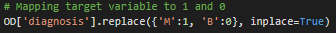
\includegraphics{object-to-int.png}

\section{Data Splitting}
    Now I need to reserve the data for classification. Since I will use 80\% of the data in my hand as a train set and 20\% as a test set, I have divided it as follows:
    \newline 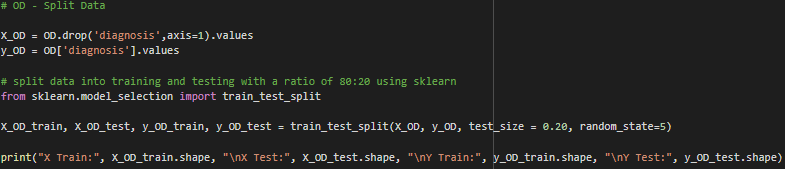
\includegraphics[scale=0.75]{OD-split.png}
    \newline I have Original Dataset (OD) dedicated train and test sets. It was also necessary to normalize this dataset according to the min-max normalization and keep it as a separate dataset (Normalized Dataset (ND)). I did it as follows:
    \newline 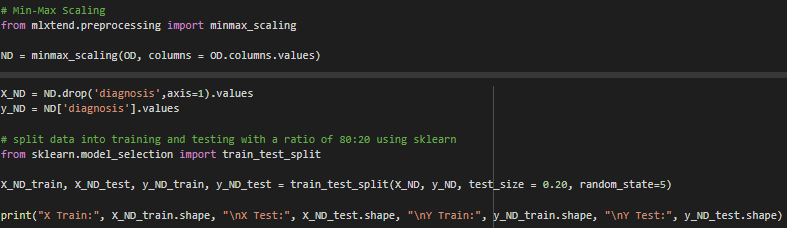
\includegraphics[scale=0.75]{ND-split.png}

\section{Clustering}
    Currently, I have OD and ND datasets. I used the K-means clustering method to cluster them. Here I have given the value of 'n\_cluster' 2, which is my class size.
    \begin{multicols}{2}
        \noindent The clustering for OD:
        \newline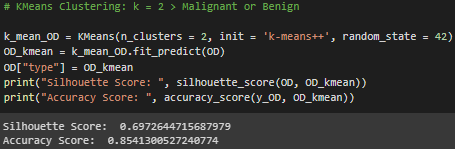
\includegraphics[scale=0.65]{cluster-od.png}
        The clustering for ND:
        \newline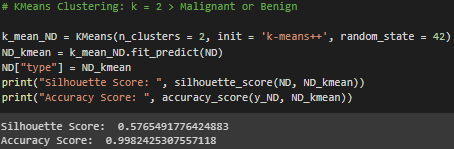
\includegraphics[scale=0.65]{cluster-nd.png}
    \end{multicols}
    \noindent Visualizing Clusters For Some Features:
    \newline 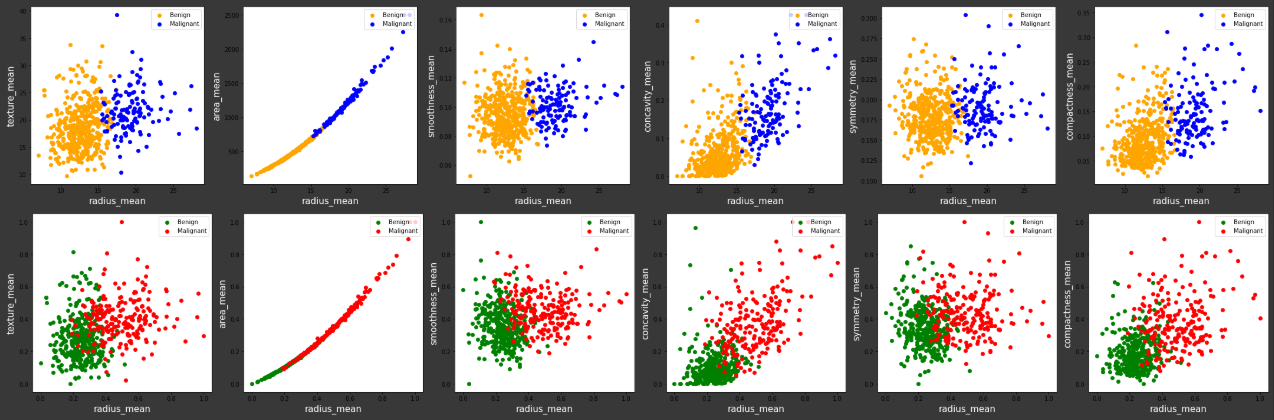
\includegraphics[scale=0.5]{clusters.png}
    \newline First Plots (orange-blue) are OD clusters. Second Plots (green-red) are ND clusters.

\section{Classification}
    I have parts of OD and ND datasets devoted to train and test datasets. I created them using the Support Vector Machine algorithm and tested them with my test data.
    \subsection{Standard Vector Machine (SVM) for OD Dataset}
    When I trained the Original Data Set with SVM, I had a nice accuracy rate of 94\%.
    \newline Confusion Matrix:
    \newline 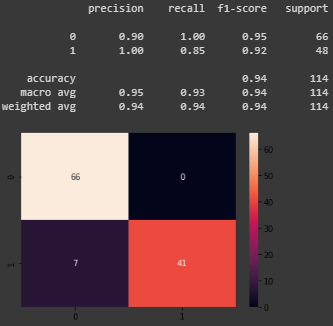
\includegraphics[scale=0.75]{confussion_od.png}
    \subsection{Standard Vector Machine (SVM) for ND Dataset}
    I achieved the highest accuracy rate of 98\% with SVM among the different classification methods I train Normalized Dataset.
    \newline Confusion Matrix:
    \newline 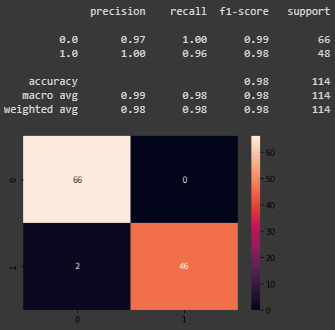
\includegraphics[scale=0.75]{confussion_nd.png}


\end{document} 
